\documentclass[12pt,a4paper]{article}
\usepackage[utf8]{inputenc}
\usepackage{fancyhdr}
%\usepackage{datetime2}
\usepackage{parskip}
\usepackage{lipsum}
\usepackage{graphicx}

\pagestyle{fancy}
\fancyhf{}

\lhead{eriro331, micso554}
\rhead{\today} % yyyy-mm-dd
\setlength{\headheight}{15pt}

\cfoot{\thepage}

\begin{document}

\begin{center}
    \Huge
    \textbf{TDDC17 - AI}

    \vspace{0.3cm}
    \Large
    Erik Rönmark
    Michael Sörsäter
    
    \vspace{0.7cm}
    \textbf{Lab2 report}
\end{center}

\textbf{1. In the vacuum cleaner domain in part 1, what were the states and actions? What is the branching factor?}

Initial state, where the agent starts. Goal state, when the agent is done. All states between are called the problem states. The actions are: move up, down, left, right and suck dirt.

The branching factor is 4.


\textbf{2. What is the difference between Breadth First Search and Uniform Cost Search in a domain where the cost of each action is 1?}

There is no difference. If actions cost can vary, then Uniform Cost Search is better.


\textbf{3. Suppose that h1 and h2 are admissible heuristics (used in for example A*). Which of the following are also admissible?
a) (h1+h2)/2
b) 2h1
c) max (h1,h2)}

Both A and C are admissible. A because h1 and h2 are both admissible and the average of them can't be greater than either h1 or h2. C because even if h2 is greater than h1, it's still admissible. 

\textbf{4. If one would use A* to search for a path to one specific square in the vacuum domain, what could the heuristic (h) be? The cost function (g)? Is it an admissible heuristic?}

H(n): An example could be the shortest straight path if ignoring obstacles from the current node to the goal node.

G(n): The cost from the initial node to the current node.

Yes, it's an admissible heuristic.

\newpage

\textbf{5. Draw and explain. Choose your three favorite search algorithms and apply them to any problem domain (it might be a good idea to use a domain where you can identify a good heuristic function). Draw the search tree for them, and explain how they proceed in the searching. Also include the memory usage. You can attach a hand-made drawing.}

\begin{figure}[ht]
	\centering
	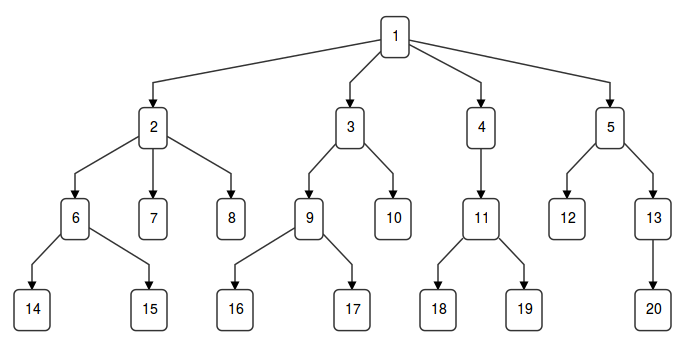
\includegraphics[width=0.9\textwidth]{graph}
    \caption{The tree used in all examples}
\end{figure}


The order for Breadth First Search: \\
1, 2, 3, 4, 5, 6, 7, 8, 9, 10, 11, 12, 13, 14, 15, 16, 17, 18, 19, 20

The order for Depth Fist Search: \\
1, 2, 6, 14, 15, 7, 8, 3, 9, 16, 17, 10, 4, 11, 18, 19, 5, 12, 13, 20

The order for 



\textbf{6. Look at all the offline search algorithms presented in chapter 3 plus A* search. Are they complete? Are they optimal? Explain why!}

\textbf{7. Assume that you had to go back and do Lab 1/Task 2 once more (if you did not use search already). Remember that the agent did not have perfect knowledge of the environment but had to explore it incrementally. Which of the search algorithms you have learned would be most suited in this situation to guide the agent's execution? What would you search for? Give an example.}



\end{document}